\chapter{Additional Topics}
%Begin Section 6.1
\section{Solving Trigonometric Equations}
An equation involving trigonometric functions is called a \emph{trigonometric
equation}.\index{trigonometric equations} For example, an equation like
\begin{displaymath}
 \tan\;A ~=~ 0.75 ~,
\end{displaymath}
which we encountered in Chapter 1, is a trigonometric equation. In Chapter 1 we were concerned only
with finding a single solution (say, between $0\Degrees$ and $90\Degrees$). In this section we will
be concerned with finding the most general solution to such equations.

To see what that means, take the above equation $\tan\;A = 0.75$. Using the
{\setlength\fboxsep{1pt}\ovalbox{\footnotesize $\tan^{-1}$}} calculator button in degree mode, we
get $A=36.87\Degrees$. However, we know that the tangent function has period $\pi$ rad
$= 180\Degrees$, i.e. it repeats every $180\Degrees$. Thus, there are many other possible answers
for the value of $A$, namely $36.87\Degrees + 180\Degrees$, $36.87\Degrees - 180\Degrees$,
$36.87\Degrees + 360\Degrees$, $36.87\Degrees - 360\Degrees$, $36.87\Degrees + 540\Degrees$, etc.
We can write this in a more compact form:
\begin{displaymath}
 A ~=~ 36.87\Degrees \;+\; 180\Degrees k \quad\text{for $k=0$, $\pm\,1$, $\pm\,2$, $...$}
\end{displaymath}
This is the most general solution to the equation.
Often the part that says ``for $k=0$, $\pm\,1$, $\pm\,2$, $...$'' is omitted since it is
usually understood that $k$ varies over all integers. The general solution in radians would be:
\begin{displaymath}
 A ~=~ 0.6435 \;+\; \pi k \quad\text{for $k=0$, $\pm\,1$, $\pm\,2$, $...$}
\end{displaymath}

\begin{exmp}
 Solve the equation $\;2\,\sin\;\theta \;+\;1 ~=~ 0$.\vspace{1mm}
 \par\noindent\textbf{Solution:} Isolating $\sin\;\theta$ gives $\;\sin\;\theta ~=~ -\tfrac{1}{2}$.
 Using the {\setlength\fboxsep{1pt}\ovalbox{\footnotesize $\sin^{-1}$}} calculator button in degree
 mode gives us $\theta = -30\Degrees$, which is in QIV. Recall that the reflection of this angle
 around the $y$-axis into QIII also has the same sine. That is, $\sin\;210\Degrees = -\tfrac{1}{2}$.
 Thus, since the sine function has period $2\pi$ rad $= 360\Degrees$, and since $-30\Degrees$ does
 not differ from $210\Degrees$ by an integer multiple of $360\Degrees$, the general solution is:
 \begin{displaymath}
  \boxed{\theta ~=~ -30\Degrees \;+\; 360\Degrees k \quad\text{and}\quad 210\Degrees \;+\;
   360\Degrees k} \qquad\text{for $k=0$, $\pm\,1$, $\pm\,2$, $...$}
 \end{displaymath}
 In radians, the solution is:
 \begin{displaymath}
  \boxed{\theta ~=~ -\dfrac{\pi}{6} \;+\; 2\pi k \quad\text{and}\quad \dfrac{7\pi}{6} + 2\pi k}
   \qquad\text{for $k=0$, $\pm\,1$, $\pm\,2$, $...$}
 \end{displaymath}
\end{exmp}
\divider
\vspace{1mm}

For the rest of this section we will write our solutions in radians.
\newpage
\begin{exmp}
 Solve the equation $\;2\cos^2 \;\theta \;-\; 1 ~=~ 0$.\vspace{1mm}
 \par\noindent\textbf{Solution:} Isolating $\;\cos^2 \;\theta$ gives us
 \begin{displaymath}
  \cos^2 \;\theta ~=~ \frac{1}{2} \quad\Rightarrow\quad \cos\;\theta ~=~ \pm\,\frac{1}{\sqrt{2}}
  \quad\Rightarrow\quad \theta ~=~ \frac{\pi}{4}\;,~\frac{3\pi}{4}\;,~\frac{5\pi}{4}\;,~
  \frac{7\pi}{4}~,
 \end{displaymath}
 and since the period of cosine is $2\pi$, we would add $2\pi k$ to each of those angles to get the
 general solution. But notice that the above angles differ by multiples of $\frac{\pi}{2}$. So since
 every multiple of $2\pi$ is also a multiple of $\frac{\pi}{2}$, we can combine those four separate
 answers into one:
 \begin{displaymath}
  \boxed{\theta ~=~ \frac{\pi}{4} \;+\; \frac{\pi}{2}\,k}
  \qquad\text{for $k=0$, $\pm\,1$, $\pm\,2$, $...$}
 \end{displaymath}
\end{exmp}
\begin{exmp}
 Solve the equation $\;2\,\sec\;\theta ~=~ 1$.\vspace{1mm}
 \par\noindent\textbf{Solution:} Isolating $\;\sec\;\theta$ gives us
 \begin{displaymath}
  \sec\;\theta ~=~ \frac{1}{2} \quad\Rightarrow\quad \cos\;\theta ~=~ \frac{1}{\sec\;\theta} ~=~ 2~,
 \end{displaymath}
 which is impossible. Thus, there is \fbox{no solution}\;.
\end{exmp}
\begin{exmp}
 Solve the equation $\;\cos\;\theta ~=~ \tan\;\theta$.\vspace{1mm}
 \par\noindent\textbf{Solution:} The idea here is to use identities to put everything in terms of a
 single trigonometric function:
 \begin{align*}
  \cos\;\theta ~&=~ \tan\;\theta\\
  \cos\;\theta ~&=~ \frac{\sin\;\theta}{\cos\;\theta}\\
  \cos^2 \;\theta ~&=~ \sin\;\theta\\
  1 \;-\; \sin^2 \;\theta ~&=~ \sin\;\theta\\
  0 ~&=~ \sin^2 \;\theta \;+\; \sin\;\theta \;-\; 1
 \end{align*}
 The last equation looks more complicated than the original equation, but notice
 that it is actually a \emph{quadratic} equation: making the substitution $x=\sin\;\theta$, we have
 \begin{displaymath}
  x^2 \;+\; x \;-\; 1 ~=~ 0 \quad\Rightarrow\quad x ~=~ \frac{-1 \;\pm\; \sqrt{1 - (4)\,(-1)}}{
   2\,(1)} ~=~ \frac{-1 \;\pm\; \sqrt{5}}{2} ~=~ -1.618\;,~0.618
 \end{displaymath}
 by the quadratic formula from elementary algebra. But $-1.618 < -1$, so it is impossible that
 $\;\sin\theta = x = -1.618$. Thus, we must have $\;\sin\;\theta = x = 0.618$. Hence, there are two
 possible solutions: $\theta = 0.666 $ rad in QI and its reflection $\pi - \theta = 2.475$
 rad around the $y$-axis in QII. Adding multiples of $2\pi$ to these gives us the general solution:
 \begin{displaymath}
  \boxed{\theta ~=~ 0.666 \;+\; 2\pi k \quad\text{and}\quad 2.475 \;+\; 2\pi k}
  \qquad\text{for $k=0$, $\pm\,1$, $\pm\,2$, $...$}
 \end{displaymath}
\end{exmp}
\divider
\newpage
\begin{exmp}
 Solve the equation $\;\sin\;\theta ~=~ \tan\;\theta$.\vspace{1mm}
 \par\noindent\textbf{Solution:} Trying the same method as in the previous example, we get
 \begin{align*}
  \sin\;\theta ~&=~ \tan\;\theta\\
  \sin\;\theta ~&=~ \frac{\sin\;\theta}{\cos\;\theta}\\
  \sin\;\theta~\cos\;\theta ~&=~ \sin\;\theta\\
  \sin\;\theta~\cos\;\theta \;-\; \sin\;\theta ~&=~ 0\\
  \sin\;\theta~(\cos\;\theta \;-\; 1) ~&=~ 0\\
  &\Rightarrow\quad \sin\;\theta ~=~ 0 \quad\text{or}\quad \cos\;\theta ~=~ 1\\
  &\Rightarrow\quad \theta ~=~ 0\;,~\pi \quad\text{or}\quad \theta ~=~ 0\\
  &\Rightarrow\quad \theta ~=~ 0\;,~\pi~,
 \end{align*}
 plus multiples of $2\pi$. So since the above angles are multiples of $\pi$, and every multiple of
 $2\pi$ is a multiple of $\pi$, we can combine the two answers into one for the general solution:
 \begin{displaymath}
  \boxed{\theta ~=~ \pi k} \qquad\text{for $k=0$, $\pm\,1$, $\pm\,2$, $...$}
 \end{displaymath}
\end{exmp}
\begin{exmp}
 Solve the equation $\;\cos\;3\theta ~=~ \frac{1}{2}$.\vspace{1mm}
 \par\noindent\textbf{Solution:} The idea here is to solve for $3\theta$ first, using the most general
 solution, and then divide that solution by $3$. So since $\;\cos^{-1} \frac{1}{2} = \frac{\pi}{3}$,
 there are two possible solutions for $3\theta$: $3\theta = \frac{\pi}{3}$ in QI and its reflection
 $-3\theta = -\frac{\pi}{3}$ around the $x$-axis in QIV. Adding multiples of $2\pi$ to these gives
 us:
 \begin{displaymath}
  3\theta ~=~ \pm\,\frac{\pi}{3} \;+\; 2\pi k \qquad\text{for $k=0$, $\pm\,1$, $\pm\,2$, $...$}
 \end{displaymath}
 So dividing everything by $3$ we get the general solution for $\theta$:
 \begin{displaymath}
  \boxed{\theta ~=~ \pm\,\frac{\pi}{9} \;+\; \frac{2\pi}{3} k}
  \qquad\text{for $k=0$, $\pm\,1$, $\pm\,2$, $...$}
 \end{displaymath}
\end{exmp}
\begin{exmp}
 Solve the equation $\;\sin\;2\theta ~=~ \sin\;\theta$.\vspace{1mm}
 \par\noindent\textbf{Solution:} Here we use the double-angle formula for sine:
 \begin{align*}
  \sin\;2\theta ~&=~ \sin\;\theta\\
  2\,\sin\theta~\cos\;\theta ~&=~ \sin\;\theta\\
  \sin\;\theta~(2\,\cos\;\theta \;-\; 1) ~&=~ 0\\
  &\Rightarrow\quad \sin\;\theta ~=~ 0 \quad\text{or}\quad \cos\;\theta ~=~ \frac{1}{2}\\
  &\Rightarrow\quad \theta ~=~ 0\;,~\pi \quad\text{or}\quad \theta ~=~ \pm\,\frac{\pi}{3}\\
  &\Rightarrow\quad \boxed{\theta ~=~ \pi k \quad\text{and}\quad \pm\,\frac{\pi}{3} \;+\; 2\pi k}
  \qquad\text{for $k=0$, $\pm\,1$, $\pm\,2$, $...$}
 \end{align*}
\end{exmp}
\divider
\newpage
\begin{exmp}\label{exmp:trigeqncombo}
\piccaption[]{\label{fig:trigeqn}}\parpic[r]{\begin{tikzpicture}[scale=0.5,
 every node/.style={font=\small}]
 \fill [fill=fillcolor] (0,0) -- (3,0) -- (3,4) -- (0,0);
 \draw (0:1.5) arc (0:53.13:1.5);
 \draw [line width=0.5pt] (2.625,0) -- (2.625,0.375) -- (3,0.375);
 \draw [linecolor,line width=1.5pt] (0,0) -- (3,0) -- (3,4) -- cycle;
 \node [below] at (1.5,0) {$2$};
 \node [right] at (3,2) {$3$};
 \node [above left] at (1.5,2) {$\sqrt{13}$};
 \node at (0.9,0.4) {$\phi$};
\end{tikzpicture}}
\noindent Solve the equation $\;2\,\sin\;\theta \;-\; 3\,\cos\;\theta ~=~ 1$.\vspace{1mm}
\par\noindent\textbf{Solution:}
We will use the technique which we discussed in Chapter 5 for finding the amplitude of a combination
of sine and cosine functions. Take the coefficients $2$ and $3$ of $\;\sin\;\theta$ and
$\;-\cos\;\theta$, respectively, in the above equation and make them the legs of a right triangle,
as in Figure \ref{fig:trigeqn}. Let $\phi$ be the angle shown in the right triangle. The leg with
length $3 >0$ means that the angle $\phi$ is above the $x$-axis, and the leg with length $2>0$ means
that $\phi$ is to the right of the $y$-axis. Hence, $\phi$ must be in QI. The hypotenuse has length
$\sqrt{13}$ by the Pythagorean Theorem, and hence $\;\cos\;\phi = \frac{2}{\sqrt{13}}$ and
$\;\sin\;\theta = \frac{3}{\sqrt{13}}$. We can use this to transform the equation to solve as
follows:
\begin{align*}
 2\,\sin\;\theta \;-\; 3\,\cos\;\theta ~&=~ 1\\
 \sqrt{13}\,\left( \tfrac{2}{\sqrt{13}}\,\sin\;\theta \;-\; \tfrac{3}{\sqrt{13}}\,\cos\;\theta
  \right) ~&=~ 1\\
 \sqrt{13}\,( \cos\;\phi\;\sin\;\theta \;-\; \sin\;\phi\;\cos\;\theta ) ~&=~ 1\\
 \sqrt{13}\,\sin\;(\theta - \phi) ~&=~ 1\quad\text{(by the sine subtraction formula)}\\
 \sin\;(\theta - \phi) ~&=~ \tfrac{1}{\sqrt{13}}\\
 &\Rightarrow\quad \theta - \phi ~=~ 0.281 \quad\text{or}\quad \theta - \phi ~=~ \pi - 0.281 = 2.861\\
 &\Rightarrow\quad \theta ~=~ \phi \;+\; 0.281 \quad\text{or}\quad \theta ~=~ \phi \;+\; 2.861
\end{align*}
Now, since $\;\cos\;\phi = \frac{2}{\sqrt{13}}$ and $\phi$ is in QI, the most general solution for
$\phi$ is $\phi = 0.983 + 2\pi k$ for $k=0$, $\pm\,1$, $\pm\,2$, $...$ . So since we needed to add
multiples of $2\pi$ to the solutions $0.281$ and $2.861$ anyway, the most general solution for
$\theta$ is:
\begin{align*}
 \theta ~&=~ 0.983 \;+\; 0.281 \;+\; 2\pi k\quad\text{and}\quad 0.983 \;+\; 2.861 \;+\; 2\pi k\\
 &\Rightarrow\quad \boxed{\theta ~=~ 1.264 \;+\; 2\pi k\quad\text{and}\quad 3.844 \;+\; 2\pi k}
\quad\text{for $k=0$, $\pm\,1$, $\pm\,2$, $...$}
\end{align*}
\end{exmp}\vspace{-4mm}
\divider
\vspace{1mm}

Note: In Example \ref{exmp:trigeqncombo} if the equation had been
$\;2\,\sin\;\theta \;+\; 3\,\cos\;\theta ~=~ 1$ then we still would have used a right triangle with
legs of lengths $2$ and $3$, but we would have used the sine addition formula
instead of the subtraction formula.

\divider
\vspace{2mm}

\startexercises\label{sec6dot1}
\vspace{2mm}
{\small
\par\noindent For Exercises 1-12, solve the given equation (in radians).
\begin{enumerate}[\bfseries 1.]
\begin{multicols}{3}
 \item $\tan\;\theta \;+\; 1 ~=~ 0$
 \item $2\,\cos\;\theta \;+\; 1 ~=~ 0$
 \item $\sin\;5\theta \;+\; 1 ~=~ 0$
\end{multicols}
\begin{multicols}{3}
 \item $2\,\cos^2 \;\theta \;-\; \sin^2 \;\theta ~=~ 1$
 \item $2\,\sin^2 \;\theta \;-\; \cos\;2\theta ~=~ 0$
 \item $2\,\cos^2 \;\theta \;+\; 3\,\sin\;\theta ~=~ 0$
\end{multicols}
\begin{multicols}{3}
 \item $\cos^2 \;\theta \;+\; 2\,\sin\;\theta ~=~ -1$
 \item $\tan\;\theta \;+\; \cot\;\theta ~=~ 2$
 \item $\sin\;\theta ~=~ \cos\;\theta$
\end{multicols}
\begin{multicols}{3}
 \item $2\,\sin\;\theta \;-\; 3\,\cos\;\theta ~=~ 0$
 \item $\cos^2 \;3\theta \;-\; 5\,\cos\;3\theta \;+\; 4 ~=~ 0$
 \item $3\,\sin\;\theta \;-\; 4\,\cos\;\theta ~=~ 1$
\end{multicols}
\end{enumerate}}
\newpage
%Begin Section 6.2
\section{Numerical Methods in Trigonometry}
We were able to solve the trigonometric equations in the previous section fairly easily, which in
general is not the case. For example, consider the equation
\begin{equation}\label{eqn:cosinefixed}
 \cos\;x ~=~ x ~.
\end{equation}
There is a solution, as shown in Figure \ref{fig:cosineeqx} below. The graphs of $y=\cos\;x$
and $y=x$ intersect somewhere between $x=0$ and $x=1$, which means that there is an $x$ in the
interval $\ival{0}{1}$ such that $\cos\;x = x$.

\begin{figure}[h]
 \begin{center}
  \input{cosineeqx.tex}\vspace{-6mm}
 \end{center}
 \caption[]{\quad $y=\cos\;x$ and $y=x$}
 \label{fig:cosineeqx}
\end{figure}

Unfortunately
there is no trigonometric identity or simple method which will help us here. Instead, we have to
resort to \emph{numerical methods}\index{numerical methods}, which provide ways of getting
successively better approximations to the actual solution(s) to within any desired degree of
accuracy. There is a large field of mathematics devoted to this subject called \emph{numerical
analysis}. Many of the methods require calculus, but luckily there is a method which we can use
that requires just basic algebra. It is called the \emph{secant method}\index{secant method}, and it
finds roots of a given function $f(x)$, i.e. values of $x$ such that $f(x)=0$. A derivation of the
secant method is beyond the scope of this book,\footnote{For an explanation of why the secant method
 works, see pp. 338-344 in \textsc{A. Ralston and P. Rabinowitz}, \emph{A First Course in Numerical
 Analysis}, 2nd ed., New York: McGraw-Hill Book Co., 1978.} but we can state the algorithm it
 uses to solve $f(x)=0$:

\begin{enumerate}[\bfseries 1.]
 \item Pick initial points $x_0$ and $x_1$ such that $x_0 < x_1$ and $f(x_0)\,f(x_1) < 0$ (i.e.
  the solution is somewhere between $x_0$ and $x_1$).
 \item For $n \ge 2$, define the number $x_n$ by
  \begin{equation}\label{eqn:secantmethod}
   x_n ~=~ x_{n-1} ~-~ \dfrac{(x_{n-1} \;-\; x_{n-2})\,f(x_{n-1})}{f(x_{n-1}) \;-\; f(x_{n-2})}
  \end{equation}
  as long as $\abs{x_{n-1} \;-\; x_{n-2}} > \epsilon_{error}$, where $\epsilon_{error} > 0$ is the
  maximum amount of error desired (usually a very small number).
 \item The numbers $x_0$, $x_1$, $x_2$, $x_3$, $...$ will approach the solution $x$ as we go through
 more iterations, getting as close as desired.
\end{enumerate}

We will now show how to use this algorithm to solve the equation $\cos\;x = x$. The solution to that
equation is the root of the function $f(x) =\cos\;x - x$. And we saw that the solution is somewhere
in the interval $\ival{0}{1}$. So pick $x_0 = 0$ and $x_1 = 1$. Then $f(0)=1$ and $f(1)=-0.4597$, so
that $f(x_0)\,f(x_1) < 0$ (we are using radians, of course). Then by definition,
\begin{align*}
 x_2 ~&=~ x_1 ~-~ \dfrac{(x_1 \;-\; x_0)\,f(x_1)}{f(x_1) \;-\; f(x_0)}\\
 &=~ 1 ~-~ \dfrac{(1 \;-\; 0)\,f(1)}{f(1) \;-\; f(0)}\\
 &=~ 1 ~-~ \dfrac{(1 \;-\; 0)\,(-0.4597)}{-0.4597 \;-\; 1}\\
 &=~ 0.6851~,\\
 x_3 ~&=~ x_2 ~-~ \dfrac{(x_2 \;-\; x_1)\,f(x_2)}{f(x_2) \;-\; f(x_1)}\\
 &=~ 0.6851 ~-~ \dfrac{(0.6851 \;-\; 1)\,f(0.6851)}{f(0.6851) \;-\; f(1)}\\
 &=~ 0.6851 ~-~ \dfrac{(0.6851 \;-\; 1)\,(0.0893)}{0.0893 \;-\; (-0.4597)}\\
 &=~ 0.7363 ~,
\end{align*}
and so on. Using a calculator is not very efficient and will lead to rounding errors. A better way
to implement the algorithm is with a computer. Listing \ref{lst:secant} below shows the code
(secant.java) for solving $\cos\;x = x$ with the secant method, using the Java programming language:

\lstset{language=Java,showstringspaces=false,lineskip=1pt,
basicstyle={\small\fontfamily{fvm}\fontseries{m}\selectfont},
columns=fullflexible,backgroundcolor=\color{codecolor},numbers=left,
numberstyle={\color{linenumcolor}\footnotesize\fontfamily{fvm}\fontseries{m}\selectfont},
commentstyle={\color{black}\small\fontfamily{fvm}\itshape\selectfont},
keywordstyle={\small\fontfamily{fvm}\fontseries{m}\selectfont},keepspaces=true,
float=h,caption={\quad Program listing for secant.java},numbersep=15pt,label=lst:secant}
\begin{center}\begin{minipage}[t]{13cm}
\begin{lstlisting}[frame=single,framerule=0pt]
import java.math.*;
public class secant {
 public static void main (String[] args) {
   double x0 =  Double.parseDouble(args[0]);
   double x1 =  Double.parseDouble(args[1]);
   double x = 0;
   double error = 1.0E-50;
   for (int i=2; i <= 10; i++) {
      if (Double.compare(Math.abs(x0 - x1),error) > 0) {
         x = x1 - (x1 - x0)*f(x1)/(f(x1) - f(x0));
         x0 = x1;
         x1 = x;
         System.out.println("x" + i + " = " + x);
      } else {
         break;
      }
   }
   MathContext mc = new MathContext(50);
   BigDecimal answer = new BigDecimal(x,mc);
   System.out.println("x = " + answer);
 }
//Define the function f(x)
 public static double f (double x) {
   return Math.cos(x) - x;
 }
}
\end{lstlisting}
\end{minipage}\end{center}

\par\noindent Lines 4-5 read in $x_0$ and $x_1$ as input parameters to the program.

\par\noindent Line 6 initializes the variable that will eventually hold the solution.

\par\noindent Line 7 sets the maximum error $\epsilon_{error}$ to be $1.0 \,\times\, 10^{-50}$. That
is, our final answer will be within that (tiny!) amount of the real solution.

\par\noindent Line 8 starts a loop of 9 iterations of the algorithm, i.e. it will create the
successive approximations $x_2$, $x_3$, $...$, $x_{10}$ to the real solution, though in Line 9 we
check to see if the two previous approximations differ by less than the maximum error. If they do,
we stop (since this means we have an acceptable solution), otherwise we continue.

\par\noindent Line 10 is the main step in the algorithm, creating $x_n$ from $x_{n-1}$ and
$x_{n-2}$.

\par\noindent Lines 11-12 set the new values of $x_{n-2}$ and $x_{n-1}$, respectively.

\par\noindent Lines 18-20 set the number of decimal places to show in the final answer
to 50 (the default is 16) and then print the answer.

\par\noindent Lines 23-24 give the definition of the function $f(x)=\cos\;x - x$.
\newpage
Below is the result of compiling and running the program using $x_0 = 0$ and $x_1 = 1$:

\begin{verbatim}
javac secant.java
java secant 0 1
x2 = 0.6850733573260451
x3 = 0.736298997613654
x4 = 0.7391193619116293
x5 = 0.7390851121274639
x6 = 0.7390851332150012
x7 = 0.7390851332151607
x8 = 0.7390851332151607
x = 0.73908513321516067229310920083662495017051696777344
\end{verbatim}

Notice that the program only got up to $x_8$, not $x_{10}$. The reason is that the difference
between $x_8$ and $x_7$ was small enough (less than $\epsilon_{error} = 1.0 \,\times\, 10^{-50}$)
to stop at $x_8$ and call that our solution.
The last line shows that solution to 50 decimal places.

Does that number look familiar? It should, since it is the answer to Exercise \ref{exer:cosxeqx} in
Section 4.1. That is, when taking repeated cosines starting with any number (in radians), you
eventually start getting the above number repeatedly after enough iterations. This turns out not to
be a coincidence. Figure \ref{fig:cosinefixed} gives an idea of why.

\begin{figure}[h]
 \begin{center}
  % GNUPLOT: LaTeX picture with Postscript
\begingroup
\footnotesize
  \makeatletter
  \providecommand\color[2][]{%
    \GenericError{(gnuplot) \space\space\space\@spaces}{%
      Package color not loaded in conjunction with
      terminal option `colourtext'%
    }{See the gnuplot documentation for explanation.%
    }{Either use 'blacktext' in gnuplot or load the package
      color.sty in LaTeX.}%
    \renewcommand\color[2][]{}%
  }%
  \providecommand\includegraphics[2][]{%
    \GenericError{(gnuplot) \space\space\space\@spaces}{%
      Package graphicx or graphics not loaded%
    }{See the gnuplot documentation for explanation.%
    }{The gnuplot epslatex terminal needs graphicx.sty or graphics.sty.}%
    \renewcommand\includegraphics[2][]{}%
  }%
  \providecommand\rotatebox[2]{#2}%
  \@ifundefined{ifGPcolor}{%
    \newif\ifGPcolor
    \GPcolortrue
  }{}%
  \@ifundefined{ifGPblacktext}{%
    \newif\ifGPblacktext
    \GPblacktexttrue
  }{}%
  % define a \g@addto@macro without @ in the name:
  \let\gplgaddtomacro\g@addto@macro
  % define empty templates for all commands taking text:
  \gdef\gplbacktext{}%
  \gdef\gplfronttext{}%
  \makeatother
  \ifGPblacktext
    % no textcolor at all
    \def\colorrgb#1{}%
    \def\colorgray#1{}%
  \else
    % gray or color?
    \ifGPcolor
      \def\colorrgb#1{\color[rgb]{#1}}%
      \def\colorgray#1{\color[gray]{#1}}%
      \expandafter\def\csname LTw\endcsname{\color{white}}%
      \expandafter\def\csname LTb\endcsname{\color{black}}%
      \expandafter\def\csname LTa\endcsname{\color{black}}%
      \expandafter\def\csname LT0\endcsname{\color[rgb]{1,0,0}}%
      \expandafter\def\csname LT1\endcsname{\color[rgb]{0,1,0}}%
      \expandafter\def\csname LT2\endcsname{\color[rgb]{0,0,1}}%
      \expandafter\def\csname LT3\endcsname{\color[rgb]{1,0,1}}%
      \expandafter\def\csname LT4\endcsname{\color[rgb]{0,1,1}}%
      \expandafter\def\csname LT5\endcsname{\color[rgb]{1,1,0}}%
      \expandafter\def\csname LT6\endcsname{\color[rgb]{0,0,0}}%
      \expandafter\def\csname LT7\endcsname{\color[rgb]{1,0.3,0}}%
      \expandafter\def\csname LT8\endcsname{\color[rgb]{0.5,0.5,0.5}}%
    \else
      % gray
      \def\colorrgb#1{\color{black}}%
      \def\colorgray#1{\color[gray]{#1}}%
      \expandafter\def\csname LTw\endcsname{\color{white}}%
      \expandafter\def\csname LTb\endcsname{\color{black}}%
      \expandafter\def\csname LTa\endcsname{\color{black}}%
      \expandafter\def\csname LT0\endcsname{\color{black}}%
      \expandafter\def\csname LT1\endcsname{\color{black}}%
      \expandafter\def\csname LT2\endcsname{\color{black}}%
      \expandafter\def\csname LT3\endcsname{\color{black}}%
      \expandafter\def\csname LT4\endcsname{\color{black}}%
      \expandafter\def\csname LT5\endcsname{\color{black}}%
      \expandafter\def\csname LT6\endcsname{\color{black}}%
      \expandafter\def\csname LT7\endcsname{\color{black}}%
      \expandafter\def\csname LT8\endcsname{\color{black}}%
    \fi
  \fi
  \setlength{\unitlength}{0.0500bp}%
  \begin{picture}(7200.00,5040.00)%
    \gplgaddtomacro\gplbacktext{%
      \csname LTb\endcsname%
      \put(946,704){\makebox(0,0)[r]{\strut{} 0}}%
      \put(946,1518){\makebox(0,0)[r]{\strut{} 0.2}}%
      \put(946,2332){\makebox(0,0)[r]{\strut{} 0.4}}%
      \put(946,3147){\makebox(0,0)[r]{\strut{} 0.6}}%
      \put(946,3961){\makebox(0,0)[r]{\strut{} 0.8}}%
      \put(946,4775){\makebox(0,0)[r]{\strut{} 1}}%
      \put(1078,484){\makebox(0,0){\strut{}$-\frac{\pi}{2}$}}%
      \put(2118,484){\makebox(0,0){\strut{}-1}}%
      \put(3941,484){\makebox(0,0){\strut{}0}}%
      \put(5763,484){\makebox(0,0){\strut{}1}}%
      \put(6803,484){\makebox(0,0){\strut{}$\frac{\pi}{2}$}}%
      \csname LTb\endcsname%
      \put(176,2739){\rotatebox{-270}{\makebox(0,0){\strut{}$y$}}}%
      \put(3940,154){\makebox(0,0){\strut{}$x$}}%
    }%
    \gplgaddtomacro\gplfronttext{%
      \csname LTb\endcsname%
      \put(1754,3961){\makebox(0,0)[l]{\strut{}$y = \cos(x)$}}%
      \put(4669,1925){\makebox(0,0)[l]{\strut{}$y = x$}}%
    }%
%    \gplgaddtomacro\gplbacktext{%
%      \put(946,704){\makebox(0,0)[r]{\strut{} 0}}%
%      \put(946,1518){\makebox(0,0)[r]{\strut{} 0.2}}%
%      \put(946,2332){\makebox(0,0)[r]{\strut{} 0.4}}%
%      \put(946,3147){\makebox(0,0)[r]{\strut{} 0.6}}%
%      \put(946,3961){\makebox(0,0)[r]{\strut{} 0.8}}%
%      \put(946,4775){\makebox(0,0)[r]{\strut{} 1}}%
%      \put(1078,484){\makebox(0,0){\strut{}$-\frac{\pi}{2}$}}%
%      \put(2118,484){\makebox(0,0){\strut{}-1}}%
%      \put(3941,484){\makebox(0,0){\strut{}0}}%
%      \put(5763,484){\makebox(0,0){\strut{}1}}%
%      \put(6803,484){\makebox(0,0){\strut{}$\frac{\pi}{2}$}}%
%      \csname LTb\endcsname%
%      \put(176,2739){\rotatebox{-270}{\makebox(0,0){\strut{}$y$}}}%
%      \put(3940,154){\makebox(0,0){\strut{}$x$}}%
%    }%
%    \gplgaddtomacro\gplfronttext{%
%      \csname LTb\endcsname%
%      \put(1754,3961){\makebox(0,0)[l]{\strut{}$y = \cos(x)$}}%
%      \put(4669,1925){\makebox(0,0)[l]{\strut{}$y = x$}}%
%    }%
%    \gplgaddtomacro\gplbacktext{%
%      \put(946,704){\makebox(0,0)[r]{\strut{} 0}}%
%      \put(946,1518){\makebox(0,0)[r]{\strut{} 0.2}}%
%      \put(946,2332){\makebox(0,0)[r]{\strut{} 0.4}}%
%      \put(946,3147){\makebox(0,0)[r]{\strut{} 0.6}}%
%      \put(946,3961){\makebox(0,0)[r]{\strut{} 0.8}}%
%      \put(946,4775){\makebox(0,0)[r]{\strut{} 1}}%
%      \put(1078,484){\makebox(0,0){\strut{}$-\frac{\pi}{2}$}}%
%      \put(2118,484){\makebox(0,0){\strut{}-1}}%
%      \put(3941,484){\makebox(0,0){\strut{}0}}%
%      \put(5763,484){\makebox(0,0){\strut{}1}}%
%      \put(6803,484){\makebox(0,0){\strut{}$\frac{\pi}{2}$}}%
%      \csname LTb\endcsname%
%      \put(176,2739){\rotatebox{-270}{\makebox(0,0){\strut{}$y$}}}%
%      \put(3940,154){\makebox(0,0){\strut{}$x$}}%
%    }%
%    \gplgaddtomacro\gplfronttext{%
%      \csname LTb\endcsname%
%      \put(1754,3961){\makebox(0,0)[l]{\strut{}$y = \cos(x)$}}%
%      \put(4669,1925){\makebox(0,0)[l]{\strut{}$y = x$}}%
%    }%
    \gplbacktext
    \put(0,0){\includegraphics{cosinefixed}}%
    \gplfronttext
  \end{picture}%
\endgroup
\vspace{-6mm}
 \end{center}
 \caption[]{\quad Attractive fixed point for $\cos\;x$}
 \label{fig:cosinefixed}
\end{figure}
%\newpage
Since $x=0.73908513321516...$ is the solution of $\cos\;x = x$, you would get
$\cos\;(\cos\;x) = \cos\;x = x$, so $\cos\;(\cos\;(\cos\;x)) = \cos\;x = x$, and so on. This number
$x$ is called an \emph{attractive fixed point} of the function $\cos\;x$. No matter where you
start, you end up getting ``drawn'' to it. Figure \ref{fig:cosinefixed} shows what happens when
starting at $x=0$: taking the cosine of $0$ takes you to $1$, and then successive cosines (indicated
by the intersections of the vertical lines with the cosine curve) eventually ``spiral'' in a
rectangular fashion to the fixed point (i.e. the solution), which is the intersection of $y=\cos\;x$
and $y=x$.\index{attractive fixed point}

Recall in Example \ref{exmp:cos6xsin4x} in Section 5.2 that we claimed that the maximum and minimum
of the function $y=\cos\;6x + \sin\;4x$ were $\pm\,1.90596111871578$, respectively. We can show this
by using the open-source program Octave.\footnote{Freely available at
\url{http://www.gnu.org/software/octave}} Octave uses a \emph{successive quadratic
 programming} method to find the minimum of a function $f(x)$. Finding the maximum of $f(x)$ is the
same as finding the minimum of $-f(x)$ then multiplying by $-1$ (why?). Below we show the commands
to run at the Octave command prompt (\texttt{octave:n>}) to find the minimum of $f(x) =
\cos\;6x + \sin\;4x$. The command \texttt{sqp(3,'f')} says to use $x=3$ as a first approximation
of the number $x$ where $f(x)$ is a minimum.
 
\begin{Verbatim}[frame=single,framesep=2mm]
octave:1> format long
octave:2> function y = f(x)
> y = cos(6*x) + sin(4*x)
> endfunction
octave:3> sqp(3,'f')
y = -1.90596111871578
ans = 2.65792064609274
\end{Verbatim}

The output says that the minimum occurs when $x=2.65792064609274$ and that the minimum is
$-1.90596111871578$. To find the maximum of $f(x)$, we find the minimum of $-f(x)$ and then take
its negative. The command \texttt{sqp(2,'f')} says to use $x=2$ as a first approximation
of the number $x$ where $f(x)$ is a maximum.

\begin{Verbatim}[frame=single,framesep=1mm]
octave:4> function y = f(x)
> y = -cos(6*x) - sin(4*x)
> endfunction
octave:5> sqp(2,'f')
y = -1.90596111871578
ans = 2.05446832062993
\end{Verbatim}

The output says that the maximum occurs when $x=2.05446832062993$
and that the maximum is $-(-1.90596111871578) = 1.90596111871578$.

Recall from Section 2.4 that Heron's formula is adequate for ``typical'' triangles, but will often
have a problem
when used in a calculator with, say, a triangle with two sides whose sum is barely larger than the
third side. However, you can get around this problem by using computer software capable of handling
numbers with a high degree of precision. Most modern computer programming languages have this
capability. For example, in the Python programming language\footnote{Available for free at
\url{http://www.python.org}} (chosen here for simplicity) the \texttt{decimal} module can be used
to set any level of precision.\footnote{Other languages have similar capability, e.g. the
\texttt{BigDecimal} class in Java.} Below we show how to get accuracy up to $50$ decimal places
using Heron's formula for the triangle in Example \ref{exmp:heronfail} from Section 2.4, by using
the python interactive command shell:

\begin{Verbatim}[frame=single,framesep=1mm]
>>> from decimal import *
>>> getcontext().prec = 50
>>> a = Decimal("1000000")
>>> b = Decimal("999999.9999979")
>>> c = Decimal("0.0000029")
>>> s = (a+b+c)/2
>>> K = s*(s-a)*(s-b)*(s-c)
>>> print Decimal(K).sqrt()
0.99999999999894999999999894874999999889618749999829
\end{Verbatim}

\noindent(Note: The triple arrow \texttt{\symbol{62}\symbol{62}\symbol{62}} is
just a command prompt, not part of the code.)\\Notice in this case that we do
get the correct answer; the high level of precision eliminates the
rounding errors shown by many calculators when using Heron's formula.

Another software option is
Sage\footnote{Visit the homepage at \url{http://www.sagemath.org} for more details.}, a
powerful and free open-source mathematics package based on Python. It can be run on your
own computer, but it can also be run through a web interface: go to \url{http://sagenb.org} to
create a free account, then once you register and sign in, click the
\textbf{New Worksheet} link to start entering commands. For example, to find the solution to
$\cos\;x = x$ in the interval $\ival{0}{1}$, enter these commands in the worksheet textfield:

\begin{Verbatim}[frame=single,framesep=1mm]
x = var('x')
find_root(cos(x) == x, 0,1)
\end{Verbatim}

\noindent Click the \textbf{evaluate} link to display the answer: $0.7390851332151559$\vspace{1mm}

\divider
\vspace{2mm}

\startexercises\label{sec6dot2}
\vspace{4mm}
{\small
\begin{enumerate}[\bfseries 1.]
 \item One obvious solution to the equation $2\,\sin\;x = x$ is $x=0$.
 Write a program to find the other solution(s), accurate to at least
 within $1.0 \,\times\, 10^{-20}$. You can use any programming language, though you may find it
 easier to just modify the code in Listing \ref{lst:secant} (only one line needs to be changed!).
 It may help to use Gnuplot to get an idea of where the graphs of $y=2\,\sin\;x$ and $y=x$
 intersect.
 \item Repeat Exercise 1 for the equation $\sin\;x = x^2$.
 \item Use Octave or some other program to find the maximum and minimum of $y=\cos\;5x - \sin\;3x$.
\end{enumerate}}
\newpage
%Begin Section 6.3
\section{Complex Numbers}
There is no real number $x$ such that $x^2 = -1$. However, it turns out to be
useful\footnote{Especially in electrical engineering, physics, and various fields of mathematics.}
to invent such a
number, called the \textbf{imaginary unit}\index{imaginary unit} and denoted by the letter $i$.
Thus, $i^2 = -1$, and hence $i = \sqrt{-1}$. If $a$ and $b$ are real numbers, then a number of the
form $a + bi$ is called a \textbf{complex number}\index{complex number}, and if $b \ne 0$ then it
is called an \textbf{imaginary number}\index{imaginary number} (and \textbf{pure
imaginary}\index{pure imaginary number}\index{imaginary number!pure} if $a=0$ and $b \ne 0$).
The real number $a$ is called the \textbf{real part}\index{real part} of the complex
number $a+bi$, and $bi$ is called its \textbf{imaginary part}\index{imaginary part}.

What does it mean to add $a$ to $bi$ in the definition $a+bi$ of a complex number, i.e. adding a
real number and an imaginary number? You can think of it as a way of \emph{extending} the set of
real numbers. If $b=0$ then $a+bi = a+0i = a$ (since $0i$ is defined as $0$), so that every real
number is a complex number.
The imaginary part $bi$ in $a+bi$ can be thought of as a way of taking the \emph{one-dimensional}
set of all real numbers and extending it to a \emph{two-dimensional} set: there is a natural
correspondence between a complex number $a+bi$ and a \emph{point} $(a,b)$ in the
(two-dimensional) $xy$-coordinate plane.

Before exploring that correspondence further, we will first state some fundamental properties of
and operations on complex numbers:

\begin{center}\statecomment{Let $a+bi$ and $c+di$ be complex numbers. Then:
\begin{enumerate}[\bfseries 1.]
 \item $a+bi ~=~ c+di$ if and only if $a=c$ and $b=d~$ (i.e. the real parts are equal and the
 imaginary parts are equal)
 \item $(a+bi) \;+\; (c+di) ~=~ (a+c) \;+\; (b+d)i~$ (i.e. add the real parts together and add the
 imaginary parts together)
 \item $(a+bi) \;-\; (c+di) ~=~ (a-c) \;+\; (b-d)i$
 \item $(a+bi)\,(c+di) ~=~ (ac-bd) \;+\; (ad+bc)i$
 \item $(a+bi)\,(a-bi) ~=~ a^2 \;+\; b^2$
 \item $\dfrac{a+bi}{c+di} ~=~ \dfrac{(ac+bd) \;+\; (bc-ad)i}{c^2 + d^2}$
\end{enumerate}}\end{center}

The first three items above are just definitions of equality, addition, and subtraction of complex
numbers. The last three items can be derived by treating the multiplication and division of complex
numbers as you would normally treat factors of real numbers:
\begin{align*}
 (a+bi)\,(c+di) ~&=~ a\,(c+di) \;+\; bi\,(c+di)\\
 &=~ ac \;+\; adi \;+\; bci \;+\; bdi^2 ~=~ ac \;+\; adi \;+\; bci \;+\; bd(-1)\\
 &=~ (ac - bd) \;+\; (ad+bc)i
\end{align*}
\newpage
\noindent The fifth item is a special case of the multiplication formula:
\begin{align*}
 (a+bi)\,(a-bi) ~&=~ ((a)(a) - (b)(-b)) \;+\; ((a)(-b) + (b)(a))i\\
 &=~ ( a^2 + b^2 ) \;+\; (-ab + ba)i ~=~ ( a^2 + b^2 ) \;+\; 0i\\
 &=~ a^2 \;+\; b^2
\end{align*}
The sixth item comes from using the previous items:
\begin{align*}
 \dfrac{a+bi}{c+di} ~&=~ \dfrac{a+bi}{c+di} \,\cdot\, \dfrac{c-di}{c-di}\\
 &=~ \dfrac{(ac - b(-d)) \;+\; (a(-d) + bc)i}{c^2 + d^2}\\
 &=~ \dfrac{(ac+bd) \;+\; (bc-ad)i}{c^2 + d^2}
\end{align*}

The \textbf{conjugate}\index{conjugate} $\overline{a+bi}$ of a complex number $a+bi$ is defined as
$\overline{a+bi} = a-bi$. Notice that $(a+bi) \;+\; \overline{(a+bi)} ~=~ 2a$ is a real number,
$(a+bi) \;-\; \overline{(a+bi)} ~=~ 2bi$ is an imaginary number if $b \ne 0$, and
$(a+bi) \overline{(a+bi)} ~=~ a^2 + b^2$ is a real number. So for a complex number $z=a+bi$,
$z\,\overline{z} = a^2 + b^2 \,$ and thus we can define the \textbf{modulus}\index{modulus} of $z$
to be $\sqrt{z\,\overline{z}} = \sqrt{a^2 + b^2}$, which we denote by $\abs{z}$.\index{complex
number!modulus of}\index{complex number!conjugate of}

\begin{exmp}
 Let $z_1 = -2+3i$ and $z_2 = 3+4i$. Find $z_1 + z_2$, $z_1 - z_2$, $z_1 \, z_2$, $z_1 / z_2$,
 $\abs{z_1}$, and $\abs{z_2}$.\vspace{1mm}
 \par\noindent\textbf{Solution:} Using our rules and definitions, we have:
 \begin{align*}
  z_1 \;+\; z_2 ~&=~ (-2+3i) \;+\; (3+4i)\\
  &=~ 1 + 7i\\
  z_1 \;-\; z_2 ~&=~ (-2+3i) \;-\; (3+4i)\\
  &=~ -5 - i\\
  z_1 \, z_2 ~&=~ (-2+3i)\, (3+4i)\\
  &=~ ((-2)(3) - (3)(4)) \;+\; ((-2)(4) + (3)(3))i\\
  &=~ -18 + i\\
  \dfrac{z_1}{z_2} ~&=~ \dfrac{-2+3i}{3+4i}\\
  &=~ \dfrac{(-2)(3) + (3)(4) \;+\; ((3)(3) - (-2)(4))i}{3^2 + 4^2}\\
  &=~ \dfrac{6}{25} \;+\; \dfrac{17}{25}\,i\\
  \abs{z_1} ~&=~ \sqrt{(-2)^2 + 3^2}\\
  &=~ \sqrt{13}\\
  \abs{z_2} ~&=~ \sqrt{3^2 + 4^2}\\
  &=~ 5
 \end{align*}
\end{exmp}
\divider
\newpage
We know that any point $(x,y)$ in the $xy$-coordinate plane that is a distance $r >0$ from the
origin has coordinates $x=r\,\cos\;\theta$ and $y=r\,\sin\;\theta$, where $\theta$ is the angle in
standard position as in Figure \ref{fig:complex}(a).

\begin{figure}[h]
 \centering
 \subfloat[][ Point $(x,y)$]{
 \begin{tikzpicture}[every node/.style={font=\small}]
  \draw [line width=0.5pt,-latex] (0.8,0) arc (0:55:0.8);
  \draw [black!60,line width=0.3pt,-latex] (-0.5,0) -- (3,0) node [right] {$x$};
  \draw [black!60,line width=0.3pt,-latex] (0,-0.5) -- (0,2.6) node [above] {$y$};
  \node [black!60,below left] at (0,0) {$0$};
  \node [right] at (30:0.4) {$\theta$};
  \draw [dashed] (0,0) -- (55:2.5) node[above left,midway] {$r$};
  \fill (55:2.5) circle (2pt) node[above right] {$(x,y)=(r\,\cos\;\theta , r\,\sin\;\theta)$};
\end{tikzpicture}}
 \qquad\qquad
 \subfloat[][ Complex number $z=x+yi$]{
 \begin{tikzpicture}[every node/.style={font=\small}]
  \draw [line width=0.5pt,-latex] (0.8,0) arc (0:55:0.8);
  \draw [black!60,line width=0.3pt,-latex] (-0.5,0) -- (3,0) node [right] {$x$};
  \draw [black!60,line width=0.3pt,-latex] (0,-0.5) -- (0,2.6) node [above] {$y$};
  \node [black!60,below left] at (0,0) {$0$};
  \node [right] at (30:0.4) {$\theta$};
  \draw [dashed] (0,0) -- (55:2.5) node[above left,midway] {$r$};
  \fill (55:2.5) circle (2pt) node[above right] {$z=x+yi = r\,\cos\;\theta\,+\,(r\,\sin\;\theta)i$};
 \end{tikzpicture}}
 \caption[]{}
 \label{fig:complex}
\end{figure}

Let $z=x+yi$ be a complex number. We can represent $z$ as a point in the \textbf{complex
plane},\index{complex plane} where the horizontal $x$-axis represents the real part of $z$, and the
vertical $y$-axis represents the pure imaginary\index{complex plane}
part of $z$, as in Figure \ref{fig:complex}(b). The distance $r$ from $z$ to the origin is, by the
Pythagorean Theorem, $r = \sqrt{x^2 + y^2}$, which is just the modulus of $z$. And we see from
Figure \ref{fig:complex}(b) that $x=r\,\cos\;\theta$ and $y=r\,\sin\;\theta$, where $\theta$ is the
angle formed by the positive $x$-axis and the line segment from the origin to $z$. We call this
angle $\theta$ the \textbf{argument}\index{argument of a complex number}\index{complex
number!argument of} of $z$. Thus, we get the
\textbf{trigonometric form}\index{trigonometric form}\index{complex number!trigonometric form}
(sometimes called the \emph{polar form}) of the complex number $z$:

\begin{center}\statecomment{For any complex number $z=x+yi$, we can write
\begin{align}
 z ~&=~ r\,(\cos\;\theta \;+\; i\,\sin\;\theta)~~,~\text{where}\label{eqn:polar}\\
 r ~&=~ \abs{z} ~=~ \sqrt{x^2 + y^2}~~\text{and}\notag\\
 \theta ~&=~ \text{the argument of $z$}~.\notag\\
 \intertext{The representation $z=r\,(\cos\;\theta \;+\; i\,\sin\;\theta)$ is often abbreviated as:}
 z ~&=~ r\,\text{cis}\;\theta\label{eqn:cis}
\end{align}}\end{center}

In the special case $z=0 = 0+0i$, the argument $\theta$ is undefined since $r=\abs{z}=0$. Also, note
that the argument $\theta$ can be replaced by $\theta \;+\; 360\Degrees k$ or $\theta \;+\; \pi k$,
depending on whether you are using degrees or radians, respectively, for $k=0$, $\pm\,1$, $\pm\,2$,
$...$ .\index{cis} Note also that for $z=x+yi$ with $r=\abs{z}$, $\theta$ must satisfy
\begin{displaymath}
 \tan\;\theta ~=~ \tfrac{y}{x}~~,~ \cos\;\theta ~=~ \tfrac{x}{r}~~,~ \sin\;\theta ~=~ \tfrac{y}{r}~.
\end{displaymath}
\newpage
\begin{exmp}
\piccaption[]{\label{fig:exmppolar}}\parpic[r]{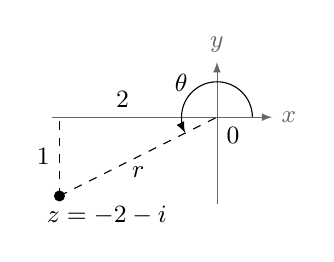
\begin{tikzpicture}[every node/.style={font=\small}]
 \draw[black!60,solid,line width=0.3pt,-latex] (-2.1,0) -- (0.7,0) node[right] {$x$};
 \draw[black!60,solid,line width=0.3pt,-latex] (0,-1.1) -- (0,0.7) node[above] {$y$};
 \node[black,below right] at (0,0) {$0$};
 \fill (-2,-1) circle (2pt);
 \draw [dashed] (-2,-1) -- (0,0) node [midway,below] {$r$};
 \draw [dashed] (-2,-1) -- (-2,0) node [midway,left] {$1$};
 \node [above] at (-1.2,0) {$2$};
 \node [below] at (-1.4,-1) {$z=-2-i$};
 \draw [-latex] (0:0.45) arc (0:206.56:0.45);
 \node [left] at (120:0.5) {$\theta$};
\end{tikzpicture}}
\noindent Represent the complex number $-2 - i$ in trigonometric form.\vspace{1mm}
 \par\noindent\textbf{Solution:} Let $z=-2-i=x+yi$, so that $x=-2$ and $y=-1$. Then $\theta$ is in
  QIII, as we see in Figure \ref{fig:exmppolar}. So since $\tan\;\theta = \tfrac{y}{x} =
  \tfrac{-1}{-2} = \tfrac{1}{2}$, we have $\theta = 206.6\Degrees$. Also,
 \begin{displaymath}
  r ~=~ \sqrt{x^2 + y^2} ~=~ \sqrt{(-2)^2 + (-1)^2} ~=~ \sqrt{5} ~.
 \end{displaymath}
 Thus, $\boxed{-2 - i = \sqrt{5}\;(\cos\;206.6\Degrees \;+\; i\,\sin\;206.6\Degrees)}\;$, or
 $\sqrt{5}\;\text{cis}\;206.6\Degrees$.
\end{exmp}
\divider
\vspace{1mm}

For complex numbers in trigonometric form, we have the following formulas for multiplication and
division:

\begin{center}\statecomment{Let $z_1 = r_1 \,(\cos\;\theta_1 \;+\; i\,\sin\;\theta_1 )$ and
$z_2 = r_2 \,(\cos\;\theta_2 \;+\; i\,\sin\;\theta_2 )$ be complex numbers. Then
\begin{align}
 z_1 \, z_2 ~&=~ r_1 \, r_2 \,(\cos\;(\theta_1 + \theta_2 ) \;+\; i\,\sin\;(\theta_1 +
  \theta_2 ))~\text{, and}\label{eqn:complextrigmult}\\
 \frac{z_1}{z_2} ~&=~ \frac{r_1}{r_2} \,(\cos\;(\theta_1 - \theta_2 ) \;+\; i\,\sin\;(\theta_1 -
  \theta_2 ))\quad\text{if $z_2 \ne 0$.}\label{eqn:complextrigdiv}
\end{align}}\end{center}

\noindent The proofs of these formulas are straightforward:
\begin{align*}
 z_1 \, z_2 ~&=~ r_1 \,(\cos\;\theta_1 \;+\; i\,\sin\;\theta_1 ) \;\cdot\;
  r_2 \,(\cos\;\theta_2 \;+\; i\,\sin\;\theta_2 )\\
 &=~ r_1 \, r_2 \,\left[ (\cos\;\theta_1 ~ \cos\;\theta_2 \;-\; \sin\;\theta_1 ~ \sin\;\theta_2 )
  \;+\; i\,(\sin\;\theta_1 ~ \cos\;\theta_2 \;+\; \cos\;\theta_1 ~ \sin\;\theta_2 ) \right]\\
 &=~ r_1 \, r_2 \,(\cos\;(\theta_1 + \theta_2 ) \;+\; i\,\sin\;(\theta_1 + \theta_2 ))\\
 \intertext{by the addition formulas for sine and cosine. And}
 \frac{z_1}{z_2} ~&=~ \frac{r_1 \,(\cos\;\theta_1 \;+\; i\,\sin\;\theta_1 )}{
  r_2 \,(\cos\;\theta_2 \;+\; i\,\sin\;\theta_2 )}\\
 &=~ \frac{r_1}{r_2} \;\cdot\; \frac{\cos\;\theta_1 \;+\; i\,\sin\;\theta_1}{
  \cos\;\theta_2 \;+\; i\,\sin\;\theta_2} \;\cdot\; \frac{\cos\;\theta_2 \;-\; i\,\sin\;\theta_2}{
  \cos\;\theta_2 \;-\; i\,\sin\;\theta_2}\\
 &=~ \frac{r_1}{r_2} \;\cdot\; \frac{(\cos\;\theta_1 ~ \cos\;\theta_2 \;+\; \sin\;\theta_1 ~
  \sin\;\theta_2 ) \;+\; i\,(\sin\;\theta_1 ~ \cos\;\theta_2 \;-\; \cos\;\theta_1 ~
  \sin\;\theta_2 )}{\cos^2 \,\theta_2 \;+\; \sin^2 \,\theta_2}\\
 &=~ \frac{r_1}{r_2} \,(\cos\;(\theta_1 - \theta_2 ) \;+\; i\,\sin\;(\theta_1 - \theta_2 ))
\end{align*}
by the subtraction formulas for sine and cosine, and since $\cos^2 \,\theta_2 \;+\;
\sin^2 \,\theta_2 = 1$. $\qed$

Note that formulas (\ref{eqn:complextrigmult}) and (\ref{eqn:complextrigdiv}) say that when
multiplying complex numbers the moduli are multiplied and the arguments are added, while when
dividing complex numbers the moduli are divided and the arguments are subtracted. This makes
working with complex numbers in trigonometric form fairly simple.
\newpage
\begin{exmp}
 Let $z_1 = 6\,(\cos\;70\Degrees \;+\; i\,\sin\;70\Degrees )$ and
 $z_1 = 2\,(\cos\;31\Degrees \;+\; i\,\sin\;31\Degrees )$. Find $z_1 \, z_2$ and
 $\frac{z_1}{z_2}$.\vspace{1mm}
 \par\noindent\textbf{Solution:} By formulas (\ref{eqn:complextrigmult}) and
 (\ref{eqn:complextrigdiv}) we have
\begin{alignat*}{3}
 z_1 \, z_2 ~&=~ (6) \, (2) \, (\cos\;(70\Degrees + 31\Degrees ) \;+\; i\,\sin\;(70\Degrees +
  31\Degrees )) \quad&&\Rightarrow\quad \boxed{z_1 \, z_2 ~=~ 12 \, (\cos\;101\Degrees \;+\;
  i\,\sin\;101\Degrees )} ~\text{, and}\\
 \frac{z_1}{z_2} ~&=~ \frac{6}{2} \, (\cos\;(70\Degrees - 31\Degrees ) \;+\; i\,\sin\;(70\Degrees -
  31\Degrees )) \quad&&\Rightarrow\quad \boxed{\frac{z_1}{z_2} ~=~ 3 \, (\cos\;39\Degrees \;+\;
  i\,\sin\;39\Degrees )} ~.
\end{alignat*}
\end{exmp}
\divider
\vspace{1mm}

For the special case when $z_1 = z_2 = z = r\,(\cos\;\theta \;+\; i\,\sin\;\theta)$ in formula
(\ref{eqn:complextrigmult}), we have
\begin{align*}
 \left[ r\,(\cos\;\theta \;+\; i\,\sin\;\theta)\right]^2 ~&=~
  r \cdot r \,(\cos\;(\theta + \theta ) \;+\; i\,\sin\;(\theta + \theta))\\
 &=~ r^2 \,(\cos\;2\theta \;+\; i\,\sin\;2\theta) ~,\\
 \intertext{and so}
 \left[ r\,(\cos\;\theta \;+\; i\,\sin\;\theta)\right]^3 ~&=~
  \left[ r\,(\cos\;\theta \;+\; i\,\sin\;\theta)\right]^2 \;\cdot\;
  r\,(\cos\;\theta \;+\; i\,\sin\;\theta )\\
 &=~ r^2 \,(\cos\;2\theta \;+\; i\,\sin\;2\theta) \;\cdot\;
  r\,(\cos\;\theta \;+\; i\,\sin\;\theta )\\
 &=~ r^3 \,(\cos\;(2\theta + \theta) \;+\; i\,\sin\;(2\theta + \theta) )\\
 &=~ r^3 \,(\cos\;3\theta \;+\; i\,\sin\;3\theta) ~,
\end{align*}
and continuing like this (i.e. by \emph{mathematical induction}), we get:\index{De Moivre's Theorem}

\statethm{thm:demoivre}{\textbf{De Moivre's Theorem:}\footnotemark \enskip For any integer $n \ge 1$,
\begin{equation}\label{eqn:demoivre}
 \left[ r\,(\cos\;\theta \;+\; i\,\sin\;\theta )\right]^n ~=~
 r^n \,(\cos\;n\theta \;+\; i\,\sin\;n\theta ) ~.
\end{equation}}\footnotetext{Named after the French statistician and mathematician Abraham de Moivre
(1667-1754).}

We define $z^0 = 1$ and $z^{-n} = 1/z^n$ for all integers $n \ge 1$. So by De Moivre's Theorem
and formula (\ref{eqn:complextrigmult}), for any $z=r\,(\cos\;\theta \;+\; i\,\sin\;\theta)$ and
integer $n \ge 1$ we get
\begin{align*}
 z^{-n} ~&=~ \frac{1}{z^n}\\
 &=~ \frac{1\,(\cos\;0\Degrees \;+\; i\,\sin\;0\Degrees )}{r^n \,(\cos\;n\theta \;+\;
  i\,\sin\;n\theta )}\\
 &=~ \frac{1}{r^n} \,(\cos\;(0\Degrees - n\theta) \;+\; i\,\sin\;(0\Degrees - n\theta))\\
 &=~ r^{-n} \, (\cos\;(- n\theta) \;+\; i\,\sin\;(- n\theta)) ~,
\end{align*}
and so De Moivre's Theorem in fact holds for \emph{all} integers.\footnote{There is a way of
defining $z^n$ when $n$ is a real (or complex) number, so that De Moivre's Theorem holds for any
real number $n$. See pp. 59-60 in \textsc{R.V. Churchill}, \emph{Complex Variables and
Applications}, 2nd ed., New York: McGraw-Hill Book Co., 1960.}
\newpage
\begin{exmp}
 Find $(1+i)^{10}$.\vspace{1mm}
 \par\noindent\textbf{Solution:} Since $1+i = \sqrt{2}\;(\cos\;45\Degrees \;+\; i\,\sin\;45\Degrees )$
 (why?), by De Moivre's Theorem we have
 \begin{displaymath}
  (1+i)^{10} ~=~ (\sqrt{2})^{10} \;(\cos\;450\Degrees \;+\; i\,\sin\;450\Degrees ) ~=~
  2^{10/2} \;(0 \;+\; i\,(1)) ~=~ 2^5 \,\cdot\, i ~=~ \boxed{32i} ~.
 \end{displaymath}
\end{exmp}
\divider
\vspace{1mm}

We can use De Moivre's Theorem to find the \emph{$n^{th}$ roots}\index{nth@$n^{th}$ roots of a
complex number}\index{complex number!$n^{th}$ roots of} of a complex number. That is, given any
complex number $z$ and positive integer $n$, find all complex numbers $w$ such that $w^n = z$.
Let $z=r\,(\cos\;\theta \;+\; i\,\sin\;\theta)$. Since the cosine and sine functions repeat every
$360\Degrees$, we know that
$z=r\,(\cos\;(\theta + 360\Degrees k)\;+\; i\,\sin\;(\theta + 360\Degrees k))$ for $k=0$, $\pm\,1$,
$\pm\,2$, $...$. Now let $w=r_0 \,(\cos\;\theta_0 \;+\; i\,\sin\;\theta_0 )$ be an $n^{th}$ root of
$z$. Then
\begin{align*}
 w^n ~=~ z \quad&\Rightarrow\quad \left[ r_0 \,(\cos\;\theta_0 \;+\; i\,\sin\;\theta_0 )\right]^n
  ~=~ r\,(\cos\;(\theta + 360\Degrees k)\;+\; i\,\sin\;(\theta + 360\Degrees k))\\
 &\Rightarrow\quad r_0^n \,(\cos\;n\theta_0 \;+\; i\,\sin\;n\theta_0 )
  ~=~ r\,(\cos\;(\theta + 360\Degrees k)\;+\; i\,\sin\;(\theta + 360\Degrees k))\\
 &\Rightarrow\quad r_0^n ~=~ r \quad\text{and}\quad n\theta_0 ~=~ \theta + 360\Degrees k\\
 &\Rightarrow\quad r_0 ~=~ r^{1/n} \quad\text{and}\quad \theta_0 ~=~
  \frac{\theta + 360\Degrees k}{n} ~.
\end{align*}
Since the cosine and sine of $\frac{\theta + 360\Degrees k}{n}$ will repeat for $k \ge n$, we get
the following formula for the $n^{th}$ roots of $z$:

\begin{center}\statecomment{For any nonzero complex number
$z=r\,(\cos\;\theta \;+\; i\,\sin\;\theta)$ and positive integer $n$, the $n$ distinct $n^{th}$
roots of $z$ are
\begin{equation}\label{eqn:nthroots}
 r^{1/n} \, \left[ \cos\;\left(\frac{\theta + 360\Degrees k}{n}\right) \;+\;
 i\,\sin\;\left(\frac{\theta + 360\Degrees k}{n}\right) \right]
\end{equation}
for $k=0$, $1$, $2$, $...$, $n-1$.}\end{center}

\noindent Note: An $n^{th}$ root of $z$ is usually written as $z^{1/n}$ or $\sqrt[n]{z}$. The number
$r^{1/n}$ in the above formula is the usual real $n^{th}$ root of the real number $r=\abs{z}$.

\begin{exmp}\label{exmp:cuberooti}
 Find the three cube roots of $i$.\vspace{1mm}
 \par\noindent\textbf{Solution:} Since $i = 1\,(\cos\;90\Degrees \;+\; i\,\sin\;90\Degrees)$, the
 three cube roots of $i$ are:
 \begin{alignat*}{3}
  \sqrt[3]{1} \;\left[ \cos\;\left(\frac{90\Degrees + 360\Degrees (0)}{3}\right) \;+\;
  i\,\sin\;\left(\frac{90\Degrees + 360\Degrees (0)}{3}\right) \right] ~&=~
  \cos\;30\Degrees \;+\; i\,\sin\;30\Degrees ~&&=~
  \boxed{\frac{\sqrt{3}}{2} \;+\; \frac{1}{2}\,i}~,\\[3pt]
  \sqrt[3]{1} \;\left[ \cos\;\left(\frac{90\Degrees + 360\Degrees (1)}{3}\right) \;+\;
  i\,\sin\;\left(\frac{90\Degrees + 360\Degrees (1)}{3}\right) \right] ~&=~
  \cos\;150\Degrees \;+\; i\,\sin\;150\Degrees ~&&=~
  \boxed{-\frac{\sqrt{3}}{2} \;+\; \frac{1}{2}\,i}~,\\[3pt]
  \sqrt[3]{1} \;\left[ \cos\;\left(\frac{90\Degrees + 360\Degrees (2)}{3}\right) \;+\;
  i\,\sin\;\left(\frac{90\Degrees + 360\Degrees (2)}{3}\right) \right] ~&=~
  \cos\;270\Degrees \;+\; i\,\sin\;270\Degrees ~&&=~ \boxed{-i}
 \end{alignat*}
\end{exmp}
\divider
\newpage
\piccaption[]{\label{fig:cuberooti}}\parpic[r]{\begin{tikzpicture}[every node/.style={font=\small}]
 \draw[black!60,solid,line width=0.3pt,-latex] (-1.4,0) -- (1.6,0) node[right] {$x$};
 \draw[black!60,solid,line width=0.3pt,-latex] (0,-1.4) -- (0,1.6) node[above] {$y$};
 \draw [line width=1pt] (0,0) circle (1.2);
 \fill [linecolor] (270:1.2) circle (2pt);
 \node [below left] at (270:1.2) {$-i$};
 \fill [linecolor] (30:1.2) circle (2pt);
 \node [right] at (30:1.2) {$\tfrac{\sqrt{3}}{2} + \tfrac{i}{2}$};
 \fill [linecolor] (150:1.2) circle (2pt);
 \node [left] at (150:1.2) {$-\tfrac{\sqrt{3}}{2} + \tfrac{i}{2}$};
 \node [above right] at (80:1.2) {$\abs{z}=1$};
 \draw [linecolor,dashed] (150:1.2) -- (0,0) -- (30:1.2);
 \draw [linecolor,dashed,latex-latex] (30:0.4) arc (30:150:0.4);
 \node [linecolor,fill=white] at (90:0.7) {$120\Degrees$};
 \draw [linecolor,dashed,latex-latex] (150:0.4) arc (150:270:0.4);
 \node [linecolor] at (210:0.8) {$120\Degrees$};
 \draw [linecolor,dashed,latex-latex] (270:0.4) arc (270:390:0.4);
 \node [linecolor] at (330:0.8) {$120\Degrees$};
\end{tikzpicture}}
Notice from Example \ref{exmp:cuberooti} that the three cube roots of $i$ are equally spaced points
along the unit circle $\abs{z}=1$ in the complex plane, as shown in Figure \ref{fig:cuberooti}.
We see that consecutive cube roots are $120\Degrees$ apart.
In general, the $n$ $n^{th}$ roots of a complex number $z$ will be equally spaced points along the
circle of radius $\abs{z}^{1/n}$ in the complex plane, with consecutive roots separated by
$\tfrac{360\Degrees}{n}$.

In higher mathematics the \emph{Fundamental Theorem of Algebra} states that every polynomial of
degree $n$ with complex coefficients has $n$ complex roots (some of which may repeat). In
particular, every real number $a$ has $n$ $n^{th}$ roots (being the roots of $z^n - a$).
For example, the square roots of $1$ are $\pm\,1$, and the square
roots of $-1$ are $\pm\,i$.

\divider
\vspace{3mm}

\startexercises\label{sec6dot3}
\vspace{5mm}
{\small
\noindent For Exercises 1-16, calculate the given expression.
\begin{enumerate}[\bfseries 1.]
\begin{multicols}{4}
 \item $(2+3i) \;+\; (-3-2i)$
 \item $(2+3i) \;-\; (-3-2i)$
 \item $(2+3i) \;\cdot\; (-3-2i)$
 \item $(2+3i)/(-3-2i)$
\end{multicols}
\begin{multicols}{4}
 \item $\overline{(2+3i)} \;+\; \overline{(-3-2i)}$
 \item $\overline{(2+3i)} \;-\; \overline{(-3-2i)}$
 \item $(1+i)/(1-i)$
 \item $\abs{-3+2i}$
\end{multicols}
\begin{multicols}{8}
 \item $i^3$
 \item $i^4$
 \item $i^5$
 \item $i^6$
 \item $i^7$
 \item $i^8$
 \item $i^9$
 \item $i^{2009}$
\end{multicols}
\suspend{enumerate}
For Exercises 17-24, prove the given identity for all complex numbers.
\resume{enumerate}[{[\bfseries 1.]}]
\begin{multicols}{4}
 \item $\overline{\left( \overline{z} \right)} \;=\; z$
 \item $\overline{z_1 + z_2} \;=\; \overline{z_1} + \overline{z_2}$
 \item $\overline{z_1 - z_2} \;=\; \overline{z_1} - \overline{z_2}$
 \item $\overline{z_1 \, z_2} \;=\; \overline{z_1} ~ \overline{z_2}$
\end{multicols}
\begin{multicols}{4}
 \item $\overline{\left( \dfrac{z_1}{z_2} \right)} \;=\; \dfrac{\overline{z_1}}{\overline{z_2}}$
 \item $\abs{z} \;=\; \abs{\overline{z}}\phantom{\dfrac{\abs{1_1}}{\abs{1_2}}}$
 \item $\abs{z_1 \, z_2} \;=\; \abs{z_1}\,\abs{z_2}\phantom{\dfrac{\abs{1_1}}{\abs{1_2}}}$
 \item $\left| \dfrac{z_1}{z_2} \right| \;=\; \dfrac{\abs{z_1}}{\abs{z_2}}$
\end{multicols}
\suspend{enumerate}
For Exercises 25-30, put the given number in trigonometric form.
\resume{enumerate}[{[\bfseries 1.]}] 
\begin{multicols}{6}
 \item $2+3i$
 \item $-3-2i$
 \item $1-i$
 \item $-i$
 \item $1$
 \item $-1$
\end{multicols}
 \item Verify that De Moivre's Theorem holds for the power $n=0$.
\suspend{enumerate}
For Exercises 32-35, calculate the given number.
\resume{enumerate}[{[\bfseries 1.]}] 
 \item $3\,(\cos\;14\Degrees \;+\; i\,\sin\;14\Degrees ) \;\cdot\;
  2\,(\cos\;121\Degrees \;+\; i\,\sin\;121\Degrees )$
\begin{multicols}{3}
 \item $\lbrack 3\,(\cos\;14\Degrees \;+\; i\,\sin\;14\Degrees )\rbrack^4\phantom{\dfrac{3}{4}}$
 \item $\lbrack 3\,(\cos\;14\Degrees \;+\; i\,\sin\;14\Degrees )\rbrack^{-4}\phantom{\dfrac{3}{4}}$
 \item $\dfrac{3\,(\cos\;14\Degrees \;+\; i\,\sin\;14\Degrees )}{
  2\,(\cos\;121\Degrees \;+\; i\,\sin\;121\Degrees )}$
\end{multicols}
\begin{multicols}{2}
 \item Find the three cube roots of $-i$.
 \item Find the three cube roots of $1+i$.
\end{multicols}
\begin{multicols}{2}
 \item Find the three cube roots of $1$.
 \item Find the three cube roots of $-1$.
\end{multicols}
\begin{multicols}{2}
 \item Find the five fifth roots of $1$.
 \item Find the five fifth roots of $-1$.
\end{multicols}
\item Find the two square roots of $-2 + 2\sqrt{3}\,i$.
\item Prove that if $z$ is an $n^{th}$ root of a real number $a$, then so is $\overline{z}$.
 (\emph{Hint: Use Exercise 20.})
\end{enumerate}}

\newpage
%Begin Section 6.4
\section{Polar Coordinates}
\piccaption[]{\label{fig:spiral}}\parpic[r]{\begin{tikzpicture}[scale=0.85,every node/.style={font=\small}]
   \draw[black!60,solid,line width=0.3pt,-latex] (-4,0) -- (4.5,0) node[right] {$x$};
   \draw[black!60,solid,line width=0.3pt,-latex] (0,-4) -- (0,3.8) node[above] {$y$};
   \node[black,below right] at (0,0) {$0$};
   \draw[linecolor,line width=1.5pt,-latex]  plot [domain=0:1080,samples=1080,smooth]
    ({(1+\x/360)*cos(\x)},{(1+(\x)/360)*sin(\x)});
   \fill (1,0) circle (2pt);
   \node [below right] at (1,0) {$1$};
   \node [below right] at (2,0) {$2$};
   \node [below right] at (3,0) {$3$};
   \draw[black!60,dashed,line width=0.3pt] (0,0) -- (145:3.8) node[black,sloped,pos=0.49,above]
    {$\gets 1 \to$} node[black,sloped,pos=0.76,above] {$\gets 1 \to$};
  \end{tikzpicture}}
Suppose that from the point $(1,0)$ in the $xy$-coordinate plane we draw a spiral around the
origin, such that the distance between any two points separated by
$360\Degrees$ along the spiral is always $1$, as in Figure \ref{fig:spiral}.
We can not express this spiral as $y=f(x)$ for some function $f$ in Cartesian coordinates, since its graph
violates the vertical rule.\index{coordinates!polar}

However, this spiral would be simple to describe using the \emph{polar coordinate
system}\index{polar coordinates}. Recall that any point $P$ distinct from the origin (denoted by
$O$) in the $xy$-coordinate plane is a distance $r>0$ from the origin, and the ray
$\overrightarrow{OP}$ makes an angle $\theta$ with the positive $x$-axis, as in Figure
\ref{fig:polar}. We call the pair $(r,\theta)$ the \textbf{polar coordinates} of $P$, and the
positive $x$-axis is called the \textbf{polar axis}\index{polar axis} of this coordinate system.
Note that $(r,\theta) = (r,\theta + 360\Degrees k)$ for $k=0$, $\pm\,1$, $\pm\,2$, $...$, so
(unlike for Cartesian coordinates) the polar coordinates of a point are not unique.

\begin{figure}[h]
\begin{minipage}[b]{7.5cm}
 \begin{center}
  \begin{tikzpicture}[every node/.style={font=\small}]
   \draw [line width=0.5pt,-latex] (0.8,0) arc (0:55:0.8);
   \draw [black!60,line width=0.3pt,-latex] (-2.2,0) -- (2.2,0) node [right] {$x$};
   \draw [black!60,line width=0.3pt,-latex] (0,-1.8) -- (0,1.8) node [above] {$y$};
   \node [black!60,below left] at (0,0) {$O$};
   \node [right] at (30:0.4) {$\theta$};
   \draw [linecolor,line width=1.5pt] (0,0) -- (55:2) node[black,above left,midway] {$r$};
   \fill (55:2) circle (2pt) node[right] {$P (r,\theta)$};
  \end{tikzpicture}\vspace{-5mm}
 \end{center}
 \caption[]{\quad Polar coordinates $(r,\theta)$}
 \label{fig:polar}
\end{minipage}
\begin{minipage}[b]{7.5cm}
 \begin{center}
  \begin{tikzpicture}[every node/.style={font=\small}]
   \draw [line width=0.5pt,-latex] (0.8,0) arc (0:55:0.8);
   \draw [black!60,line width=0.3pt,-latex] (-2.2,0) -- (2.2,0) node [right] {$x$};
   \draw [black!60,line width=0.3pt,-latex] (0,-1.8) -- (0,1.8) node [above] {$y$};
   \node [black!60,below right] at (0,0) {$O$};
   \node [right] at (30:0.4) {$\theta$};
   \draw [dashed] (0,0) -- (55:2);
   \draw [linecolor,line width=1.5pt] (0,0) -- (235:2) node[black,above left,midway] {$-r$};
   \fill (235:2) circle (2pt) node[left] {$P (-r,\theta)$};
  \end{tikzpicture}\vspace{-5mm}
 \end{center}
 \caption[]{\quad Negative $r$: $(-r,\theta)$}
 \label{fig:negpolar}
\end{minipage}
\end{figure}

In polar coordinates we adopt the convention that $r$ can be negative, by defining $(-r,\theta) =
(r,\theta + 180\Degrees)$ for any angle $\theta$. That is, the ray $\overrightarrow{OP}$ is drawn in
the opposite direction from the angle $\theta$, as in Figure \ref{fig:negpolar}. When $r=0$, the
point $(r,\theta) = (0,\theta)$ is the origin $O$, regardless of the value of $\theta$.

You may be familiar with graphing paper, for plotting points or functions given in Cartesian
coordinates (sometimes also called
\emph{rectangular coordinates}).\index{rectangular coordinates}\index{coordinates!rectangular}
Such paper consists of a rectangular grid. Similar graphing paper exists for plotting points and
functions in polar coordinates, similar to Figure \ref{fig:polargraph}.
\newpage
\begin{figure}[h]
 \begin{center}
  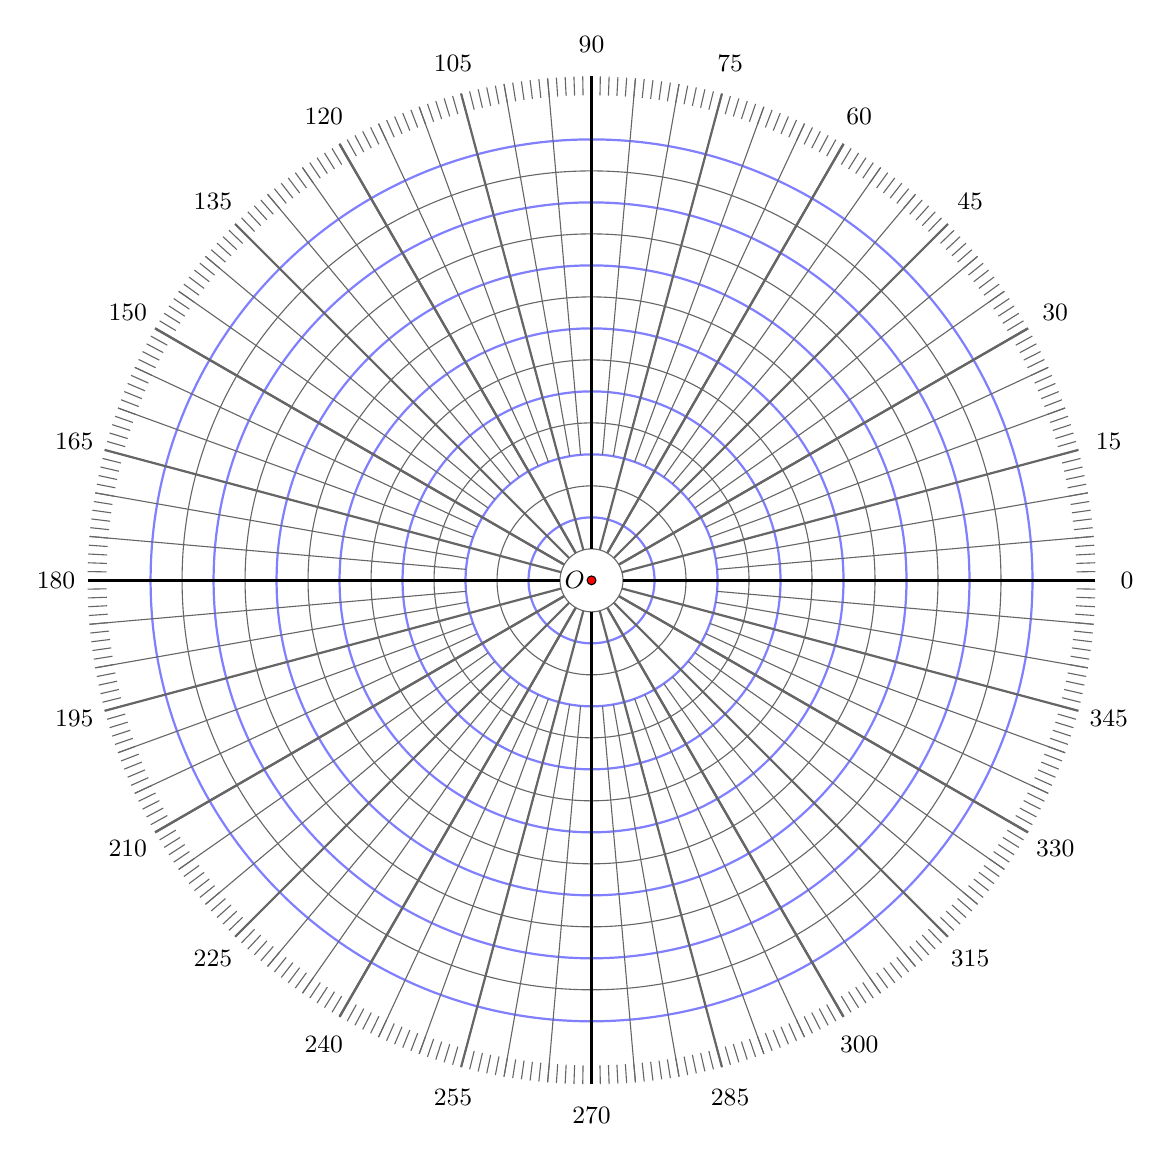
\begin{tikzpicture}[scale=0.8,every node/.style={font=\small}]
   \foreach \r in {1, 2,...,7}
     \draw[blue!50,thick] (0,0) circle (\r);    
   \foreach \r in {0.5, 1.5,...,7}
     \draw[black!60, thin] (0,0) circle (\r);
   \foreach \a in {0, 1,...,359}
     \draw[black!60,thin] (\a:7.7) -- (\a:8);
   \foreach \a in {0, 5,...,355}
     \draw[black!60] (\a:2) -- (\a:8);      
   \foreach \a in {0, 15,...,345}
     \draw[thick,black!60] (\a:0.5) -- (\a:8); 
   \foreach \a in {0, 30,...,330}
     \draw[thick,black!60] (\a:0.5) -- (\a:8);
   \foreach \a in {0, 90,...,270}
     \draw[very thick] (\a:0.5) -- (\a:8);
   \foreach \a in {0, 15,...,345}
     \draw (\a: 8.5) node {$\a\Degrees$};
   \draw[fill=red] (0,0) circle(0.7mm);
   \node [left] at (0.05,0) {$O$};
  \end{tikzpicture}
 \end{center}
 \caption[]{\quad Polar coordinate graph}
 \label{fig:polargraph}
\end{figure}

The angle $\theta$ can be given in either degrees or radians, whichever is more convenient. Radians
are often preferred when graphing functions in polar coordinates. The reason is that, 
unlike degrees, radians can be considered ``unitless'' (as we mentioned in
Chapter 4). This is desirable when a function
given in polar coordinates is expressed as $r$ as a function of $\theta$ (similar to how, in Cartesian
coordinates $(x,y)$, functions are usually expressed as $y$ as a function of $x$). For example, if a
function in polar coordinates is written as $r = 2\,\theta$, then $r$ would have the same units as
$\theta$. But $r$ should be a unitless quantity, hence using radians for $\theta$ makes more sense
in this case.
\newpage
\begin{exmp}
 Express the spiral from Figure \ref{fig:spiral} in polar coordinates.\vspace{1mm}
 \par\noindent\textbf{Solution:} We will use radians for $\theta$. The goal is to find some equation
 involving $r$ and $\theta$ that describes the spiral. We see that
 \begin{align*}
  \theta ~=~ 0 \quad&\Rightarrow\quad r ~=~ 1\\
  \theta ~=~ 2\pi \quad&\Rightarrow\quad r ~=~ 2\\
  \theta ~=~ 4\pi \quad&\Rightarrow\quad r ~=~ 3\\
  &\vdots\\
  \theta ~=~ 2\pi\,k \quad&\Rightarrow\quad r ~=~ 1+k\\
 \end{align*}
 for $k=0,1,2,\ldots$. In fact, that last relation holds for any nonnegative real number $k$ (why?).
 So for any $\theta \ge 0$,
 \begin{displaymath}
  \theta ~=~ 2\pi\,k \quad\Rightarrow\quad k ~=~ \frac{\theta}{2\pi} \quad\Rightarrow\quad r ~=~
  1 + k ~=~ 1 + \frac{\theta}{2\pi} ~.
 \end{displaymath}
 Hence, the spiral can be written as $\boxed{r ~=~ 1 + \frac{\theta}{2\pi}}$ for $\theta \ge 0$. The
 graph is shown in Figure \ref{fig:spiralgnu}, along with the Gnuplot commands to create the graph.

\piccaption[]{\quad $r = 1 + \frac{\theta}{2\pi}$\label{fig:spiralgnu}}\parpic[r]{
\scalebox{0.90}{\input{spiral.tex}}}
\begin{verbatim}
set polar
set size square
set samples 2000
unset key
set zeroaxis
set xlabel "x"
set ylabel "y"
plot [0:6*pi] 1 + t/(2*pi)
\end{verbatim}\vspace{-30mm}
\picskip{0}
Note that when using the \texttt{set polar} command, Gnuplot will assume that the function being
plotted is $r$ as a function of $\theta$ (represented by the variable \texttt{t} in Gnuplot).
\end{exmp}\vspace{-1mm}
\divider
\newpage
\piccaption[]{\label{fig:polarconvert}}\parpic[r]{\begin{tikzpicture}[every node/.style={font=\small}]
 \draw [line width=0.5pt,-latex] (0.8,0) arc (0:55:0.8);
 \draw [black!60,line width=0.3pt,-latex] (-0.5,0) -- (2.2,0) node [right] {$x$};
 \draw [black!60,line width=0.3pt,-latex] (0,-0.5) -- (0,1.8) node [above] {$y$};
 \node [black!60,below left] at (0,0) {$O$};
 \node [right] at (30:0.4) {$\theta$};
 \draw [dashed] (1.1472,0) -- (1.1472,1.6383);
 \draw [snake=brace,segment amplitude=3mm] (1.3,1.6383) -- (1.3,0);
 \draw [snake=brace,segment amplitude=3mm] (1.1472,-0.1)-- (0,-0.1);
 \node[right] at (1.55,0.81915) {$y$};
 \node[below] at (0.5736,-0.35) {$x$};
 \draw [linecolor,line width=1.5pt] (0,0) -- (55:2) node[black,above left,midway] {$r$};
 \fill (55:2) circle (2pt) node[above right] {$(r,\theta)$} node[above left] {$(x,y)$};
\end{tikzpicture}}
Figure \ref{fig:polarconvert} shows how to convert between polar coordinates and Cartesian
coordinates. For a point with polar coordinates $(r,\theta)$ and Cartesian coordinates $(x,y)$:

\noindent\textbf{Polar to Cartesian:}
\begin{equation}\label{eqn:polartorect}
 \boxed{ x ~=~ r\,\cos\;\theta \qquad y ~=~ r\,\sin\;\theta }
\end{equation}

\noindent\textbf{Cartesian to Polar:}
\begin{equation}\label{eqn:recttopolar}
 \boxed{ r ~=~ \pm\;\sqrt{x^2 ~+~ y^2} \qquad \tan\;\theta ~=~ \frac{y}{x} ~~\text{if $x \ne 0$} }
\end{equation}\vspace{-2mm}
\picskip{0}
Note that in formula (\ref{eqn:recttopolar}), if $x = 0$ then $\theta = \pi/2$ or $\theta = 3\pi/2$.
Also, if $x \ne 0$ and $y \ne 0$ then the two possible solutions for $\theta$ in the equation
$\tan\;\theta ~=~ \frac{y}{x}$ are in opposite quadrants (for $0 \le \theta < 2\pi$). If the angle
$\theta$ is in the same quadrant as the point $(x,y)$, then $r = \sqrt{x^2 ~+~ y^2}$ (i.e. $r$ is
positive); otherwise $r = -\sqrt{x^2 ~+~ y^2}$ (i.e. $r$ is negative).

\begin{exmp}
Convert the following points from polar coordinates to Cartesian coordinates:\\
\textbf{(a)} $(2,30\Degrees)$; \textbf{(b)} $(3,3\pi/4)$; \textbf{(c)} $(-1,5\pi/3)$\vspace{1mm}
\par\noindent\textbf{Solution:} \textbf{(a)} Using formula (\ref{eqn:polartorect}) with $r=2$ and
$\theta = 30\Degrees$, we get:
\begin{displaymath}
 (x,y) ~=~ ( r\,\cos\;\theta, r\,\sin\;\theta) ~=~ (2\,\cos\;30\Degrees,2\,\sin\;30\Degrees) ~=~
 \left(2 \;\cdot\; \tfrac{\sqrt{3}}{2}, 2 \;\cdot\; \tfrac{1}{2} \right) \quad\Rightarrow\quad
 \boxed{(x,y) ~=~ \left( \sqrt{3},1 \right)}
\end{displaymath}
 \par\noindent\textbf{(b)} Using formula (\ref{eqn:polartorect}) with $r=3$ and
 $\theta = 3\pi/4$, we get:
\begin{displaymath}
 (x,y) ~=~ ( r\,\cos\;\theta, r\,\sin\;\theta) ~=~ \left( 3\,\cos\;\tfrac{3\pi}{4},3\,\sin\;\tfrac{3\pi}{4}
 \right) ~=~ \left(3 \;\cdot\; \tfrac{-1}{\sqrt{2}}, 3 \;\cdot\; \tfrac{1}{\sqrt{2}} \right)
 \quad\Rightarrow\quad \boxed{(x,y) ~=~ \left( \tfrac{-3}{\sqrt{2}},\tfrac{3}{\sqrt{2}} \right)}
\end{displaymath}
 \par\noindent\textbf{(c)} Using formula (\ref{eqn:polartorect}) with $r=-1$ and
 $\theta = 5\pi/3$, we get:
\begin{displaymath}
 (x,y) ~=~ ( r\,\cos\;\theta, r\,\sin\;\theta) ~=~ \left( -1\,\cos\;\tfrac{5\pi}{3},-1\,\sin\;\tfrac{5\pi}{3}
 \right) ~=~ \left(-1 \;\cdot\; \tfrac{1}{2},-1 \;\cdot\; \tfrac{-\sqrt{3}}{2} \right)
 \quad\Rightarrow\quad \boxed{(x,y) ~=~ \left( -\tfrac{1}{2},\tfrac{\sqrt{3}}{2} \right)}
\end{displaymath}
\end{exmp}
\begin{exmp}
Convert the following points from Cartesian coordinates to polar coordinates:\\
\textbf{(a)} $(3,4)$; \textbf{(b)} $(-5,-5)$\vspace{1mm}
\par\noindent\textbf{Solution:} \textbf{(a)} Using formula (\ref{eqn:recttopolar}) with $x=3$ and
$y=4$, we get:
\begin{displaymath}
 \tan\;\theta ~=~ \frac{y}{x} ~=~ \frac{4}{3} \quad\Rightarrow\quad \theta ~=~ 53.13\Degrees \quad
 \text{or}\quad \theta ~=~ 233.13\Degrees
\end{displaymath}
Since $\theta = 53.13\Degrees$ is in the same quadrant (QI) as the point $(x,y) = (3,4)$, we can
take\\$r ~=~ \sqrt{x^2 + y^2} = \sqrt{3^2 + 4^2} = 5$. Thus, $\boxed{(r,\theta) = (5,53.13\Degrees)}$~.

\noindent Note that if we had used $\theta = 233.13\Degrees$, then we would have $(r,\theta) =
(-5,233.13\Degrees)$.

\par\noindent\textbf{(b)}  Using formula (\ref{eqn:recttopolar}) with $x=-5$ and $y=-5$, we get:
\begin{displaymath}
 \tan\;\theta ~=~ \frac{y}{x} ~=~ \frac{-5}{-5} ~=~ 1 \quad\Rightarrow\quad \theta ~=~ 45\Degrees \quad
 \text{or}\quad \theta ~=~ 225\Degrees
\end{displaymath}
Since $\theta = 225\Degrees$ is in the same quadrant (QIII) as the point $(x,y) = (-5,-5)$, we can
take\\$r ~=~ \sqrt{x^2 + y^2} = \sqrt{(-5)^2 + (-5)^2} = 5\,\sqrt{2}$. Thus, $\boxed{(r,\theta) =
(5\,\sqrt{2},225\Degrees)}$~.

\noindent Note that if we had used $\theta = 45\Degrees$, then we would have $(r,\theta) =
(-5\,\sqrt{2},45\Degrees)$.
\end{exmp}
\begin{exmp}\label{exmp:polarcircle}
 Write the equation $x^2 + y^2 = 9$ in polar coordinates.\vspace{1mm}
 \par\noindent\textbf{Solution:} This is just the equation of a circle of radius $3$ centered at the
 origin. Since $r = \pm\sqrt{x^2 + y^2} = \pm\sqrt{9}$, in polar coordinates the equation can be written
 as simply $\boxed{r = 3}$~.
\end{exmp}
\begin{exmp}
 Write the equation $x^2 + (y-4)^2 = 16$ in polar coordinates.\vspace{1mm}
 \par\noindent\textbf{Solution:} This is the equation of a circle of radius $4$ centered at the point
 $(0,4)$. Expanding the equation, we get:
 \begin{align*}
  x^2 ~+~ (y-4)^2 ~&=~ 16\\
  x^2 ~+~ y^2 ~-~ 8y ~+~ 16 ~&=~ 16\\
  x^2 ~+~ y^2 ~&=~ 8y\\
  r^2 ~&=~ 8\,r\sin\;\theta\\
  r ~&=~ 8\,\sin\;\theta
 \end{align*}
 Why could we cancel $r$ from both sides in the last step? Because we know that the point $(0,0)$
 is on the circle, so canceling $r$ does not eliminate $r=0$ as a potential solution of the
 equation (since $\theta = 0\Degrees$ would make $r = 8\,\sin\;\theta = 8\,\sin\;0\Degrees = 0$). Thus,
 the equation is $\boxed{r = 8\,\sin\;\theta}$~.
\end{exmp}
\begin{exmp}
 Write the equation $y = x$ in polar coordinates.\vspace{1mm}
 \par\noindent\textbf{Solution:} This is the equation of a line through the origin. So when $x=0$, we
 know that $y=0$. When $x \ne 0$, we get:
 \begin{align*}
  y ~&=~ x\\
  \frac{y}{x} ~&=~ 1\\
  \tan\;\theta ~&=~ 1\\
  \theta ~&=~ 45\Degrees
 \end{align*}
Since there is no restriction on $r$, we could have $r=0$ and $\theta = 45\Degrees$, which would take care
of the case $x = 0$ (since then $(x,y) = (0,0)$, which is the same as $(r,\theta) = (0,45\Degrees))$. Thus,
the equation is $\boxed{\theta = 45\Degrees}$~.
\end{exmp}\vspace{-1mm}
\divider\vspace{-2mm}
\newpage
\begin{exmp}
 Prove that the distance $d$ between two points $(r_1 , \theta_1)$ and $(r_2 , \theta_2)$ in polar
 coordinates is
 \begin{equation}\label{eqn:polardist}
  d ~=~ \sqrt{r_1^2 ~+~ r_2^2 ~-~ 2r_1r_2\,\cos\;(\theta_1 - \theta_2)} ~~.
 \end{equation}
 \par\noindent\textbf{Solution:} The idea here is to use the distance formula in Cartesian coordinates,
 then convert that to polar coordinates. So write
 \begin{alignat*}{4}
  x_1 ~&=~ r_1 \,\cos\;\theta_1 \qquad& y_1 ~&=~ r_1 \,\sin\;\theta_1\\
  x_2 ~&=~ r_2 \,\cos\;\theta_2 \qquad& y_2 ~&=~ r_2 \,\sin\;\theta_2 ~.
 \end{alignat*}
 Then $(x_1,y_1)$ and $(x_2,y_2)$ are the Cartesian equivalents of $(r_1 , \theta_1)$ and $(r_2 , \theta_2)$,
 respectively. Thus, by the Cartesian coordinate distance formula,
 \begin{align*}
  d^2 ~&=~ (x_1 - x_2)^2 ~+~ (y_1 - y_2)^2\\
  &=~ (r_1 \,\cos\;\theta_1 - r_2 \,\cos\;\theta_2)^2 ~+~ (r_1 \,\sin\;\theta_1 - r_2 \,\sin\;\theta_2)^2\\
  &=~ r_1^2 \cos^2\;\theta_1 ~-~ 2r_1 r_2 \cos\;\theta_1~\cos\;\theta_2 ~+~ r_2^2 \cos^2\;\theta_2 ~+~
   r_1^2 \sin^2\;\theta_1 ~-~ 2r_1 r_2 \sin\;\theta_1~\sin\;\theta_2 ~+~ r_2^2 \sin^2\;\theta_2\\
  &=~ r_1^2 (\cos^2\;\theta_1 ~+~ \sin^2\;\theta_1) ~+~ r_2^2 (\cos^2\;\theta_2 ~+~ \sin^2\;\theta_2) ~-~
   2r_1 r_2 (\cos\;\theta_1~\cos\;\theta_2 ~+~ \sin\;\theta_1~\sin\;\theta_2)\\
  d^2 ~&=~ r_1^2 ~+~ r_2^2 ~-~ 2r_1r_2\,\cos\;(\theta_1 - \theta_2) ~,
 \end{align*}
 so the result follows by taking square roots of both sides.
\end{exmp}\vspace{-1mm}
\divider
\vspace{2mm}

In Example \ref{exmp:polarcircle} we saw that the equation $x^2 + y^2 = 9$ in Cartesian coordinates
could be expressed as $r = 3$ in polar coordinates. This equation describes a circle centered at the
origin, so the circle is symmetric about the origin. In general, polar coordinates are useful in
situations when there is symmetry about the origin (though there are other situations), which arise
in many physical applications.

\divider
\vspace{2mm}

\startexercises\label{sec6dot4}
\vspace{5mm}
{\small
\par\noindent For Exercises 1-5, convert the given point from polar coordinates to Cartesian
coordinates.
\begin{enumerate}[\bfseries 1.]
\begin{multicols}{5}
 \item $(6,210\Degrees)$
 \item $(-4,3\pi)$
 \item $(2,11\pi/6)$
 \item $(6,90\Degrees)$
 \item $(-1,405\Degrees)$
\end{multicols}
\suspend{enumerate}
For Exercises 6-10, convert the given point from Cartesian coordinates to polar coordinates.
\resume{enumerate}[{[\bfseries 1.]}]
\begin{multicols}{5}
 \item $(3,1)$
 \item $(-1,-3)$
 \item $(0,2)$
 \item $(4,-2)$
 \item $(-2,0)$
\end{multicols}
\suspend{enumerate}
For Exercises 11-18, write the given equation in polar coordinates.
\resume{enumerate}[{[\bfseries 1.]}]
\begin{multicols}{4}
 \item $(x-3)^2 + y^2 = 9$
 \item $y = -x$
 \item $x^2 - y^2 = 1$
 \item $3x^2 + 4y^2 - 6x = 9$
\end{multicols}
\item Graph the function $r = 1 + 2\,\cos\;\theta$ in polar coordinates.
\end{enumerate}}
